% ChapterPub1

%\label{ChapterPub1} % For referencing the chapter elsewhere, use \ref{ChapterPub1} 

%\lhead{Chapter 2. \emph{Methods}} % This is for the header on each page - perhaps a shortened title

\pagestyle{empty}

\addtocontents{toc}{\cftpagenumbersoff{chapter}}



\centering{
\setcounter{chapter}{0}
\chapter{Wolfisberg et al., Journal of Virological Methods, 2013}

\bigskip
\bigskip
\bigskip
\bigskip

\LARGE{\textbf{Impaired genome encapsidation restricts the \textit{in vitro} propagation of human parvovirus B19.}}

\bigskip
\bigskip
\bigskip

Raphael Wolfisberg, Nico Ruprecht, Christoph Kempf and Carlos Ros}


\phantomsection\addcontentsline{toc}{section}{Impaired genome encapsidation restricts the \textit{in vitro} propagation of human parvovirus B19.}



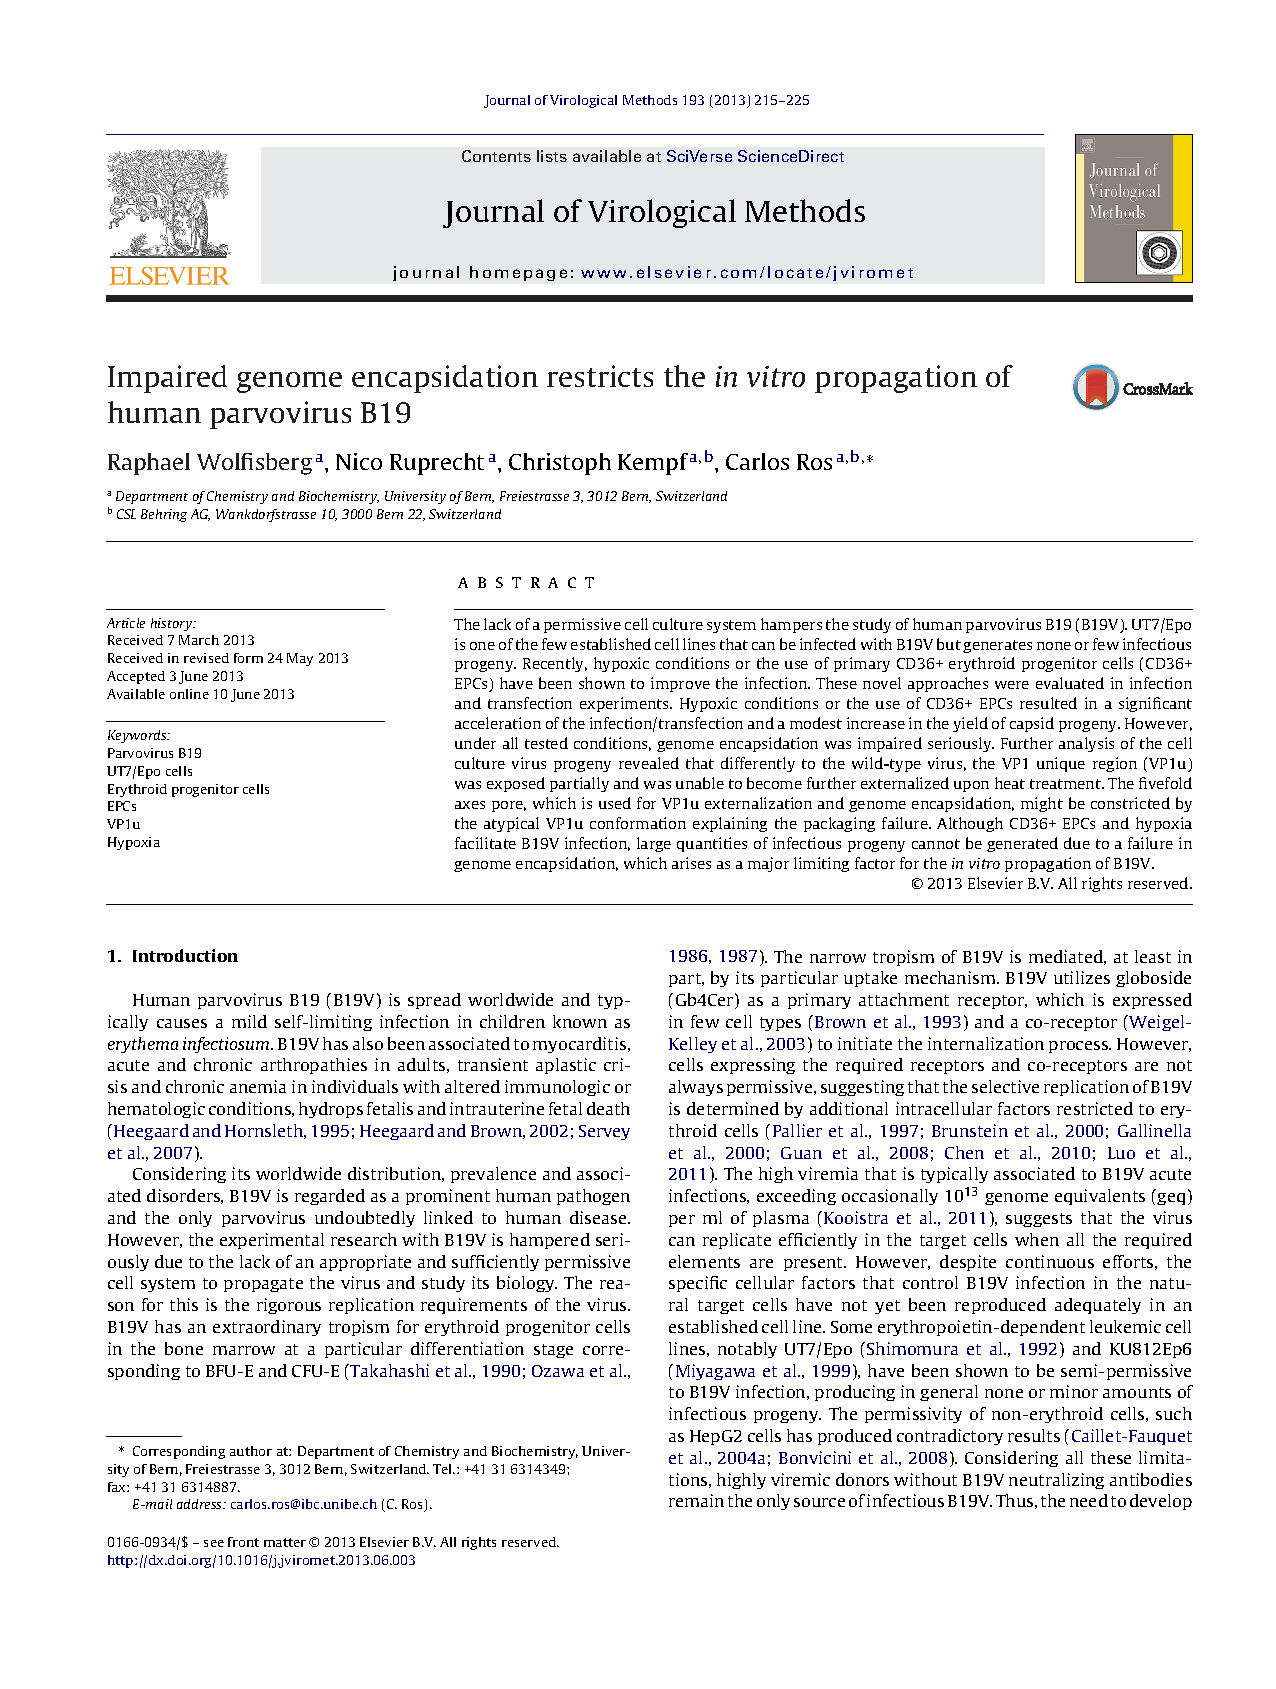
\includepdf[pagecommand=\thispagestyle{empty}, pages={1-11}, scale=0.9]{../pdfdocuments/b19vpaper}



